\chapter{Reducing FCT with flow prioritization}

To the purpose of minimizing the average flow completion time (FCT), a common strategy is to treat short flows with tight latency constraints differently from the others. This can be managed with prioritization and scheduling algorithms, for which there already exist numerous theoretical studies. In the following of this chapter will be reviewed the most significant of them, with care to their application to datacenter networks. 

\section{Theoretical scheduling background}
At high level, scheduling policies can be classified into two categories, depending whether or not flow properties --- such as size and deadline --- are known a priori.

\subsection{Flow-aware disciplines}
Flow-aware disciplines are those techniques that assumes the job characteristics are precisely known before initiation. While this is often the case for many systems in other industries like manufacturing, it is not always so in communication networks. Sometimes the flow size is known exactly, for example when a server is requested a static object (e.g. a static Web page, a file transfer) or it can be roughly estimated, but generally speaking this information is either not available or it involves undesired modifications of the application layer. \\
The optimal approach to minimize the job completion time for an offline system is the \emph{Shortest Job First} (SJF) discipline that consists in serving jobs in decreasing order with respect to their size. However this policy is not suitable for dynamic contexts where new jobs can arrive at any time instant. For such scenarios has been adopted a preemptive version of SJF, known as \emph{Shortest Remaining Processing Time} (SRPT), which chooses first the job with shortest time left to its completion, or equivalently in the context of flow scheduling, the smallest amount of bytes left. SRPT has been proven for long to be the optimal policy for minimizing the average response time (i.e. FCT) in a single server system, regardless of the serving time and inter-arrival distribution \cite{schrage_1968}. 
%however it can excessively penalize large flows with a protracted starvation. 
%However, its performances on long flows depend on the job size distribution and in particular for heavy-tailed distributions also long flows experience lower completion time in respect to the simple Processor Sharing (PS) policy. Thus, the fact that in a datacenter network the majority of flows are short, but nearly all bytes are carried by few elephants, makes this strategy very attractive.

\subsection{Flow-agnostic disciplines}
\label{sec:las}
In absence of precise knowledge about the flow length, a very effective policy is the dual approach to SRPT, the so called \emph{Least Attained Service} (LAS) or \emph{Foreground-Background} (FB). LAS is a preemptive scheduler which gives service first to the flow that has transmitted less bytes, serving in processor sharing when there are ties among flows. In other words, a job retains alone the processor until it is has received the same service of another jobs in the system or it is preempted by a newly arrived shorter job. If no fresh jobs arrive, those in the systems prosecute sharing the processor. The main insight of LAS is to exploit the increasing knowledge about the flow size gained during its service. In fact, the LAS scheduler becomes more and more confident that a given flow is a large one, as further of its bytes are transmitted. 

LAS is optimal among the flow-agnostic disciplines when the hazard rate of the flow size distribution is a  decreasing function \cite{Gittins}. The hazard rate is defined as the ratio of the probability density function $f_X(x)$ to the survival function:
\[
	h(x) = \dfrac{f_X(x)}{1-F_X(x)}
\]  and it is a function that represents the instantaneous failure rate of a quantity. For instance, it can be seen as the likelihood that the flow size $X$ ends at value $x$ given that $x$ bytes have already been observed. As a general rule, heavy-tailed distributions exhibit a decreasing $h(x)$, whereas $h(x)$ is increasing for light-tailed distributions and constant for the exponential distribution. Thus, LAS works at best under job size distributions that present high variability, which is a case of interest since they well model datacenter's traffic where a majority of short flows coexists with few very large flows. 

At this point, it is interesting to better understand how LAS compares to other disciplines, such as PS, not only on average but in depth with respect to flow sizes, in order to quantify its impact on small and large jobs. Also, it would be useful to bound the sub-optimality of LAS with respect to the SRPT flow-aware scheduler.  To this purpose, the authors of \cite{LAS_analysis} compared different distributions with increasing coefficients of variation, under LAS, PS and SRPT disciplines.  The \emph{coefficient of variation} C, is a single number measure of the variability of a distribution and it is expressed as the standard deviation $\sigma$ normalized to the mean of the distribution $\mu$: 

\[
 C = \dfrac{\sigma}{\mu}
\] The comparison was based on the \emph{average conditional completion time}, that is the average completion time of flows belonging to a given size. Formally, denoting as $T$ the random variable associated to the completion time and X as the random variable associated to the flow size, the average conditional completion time is defined as $\mathbb{E}[T | X = x]$. This is a rather practical quantity to tell how the FCT vary with flow sizes and to highlight unfairnesses brought by the scheduling policy.

The distributions taken into account were the negative exponential distribution, whose probability density function rapidly converges to zero, and a set of Bounded Pareto distributions with varying $C$, as example of heavy-tailed distributions. Their probability density functions are given by:

\begin{align*}
	& f(x)_{Exp} = u(x) \mu e^{-\mu x}, & \qquad \mu \geq 0 \\
	& f(x)_{BP} = \frac{\alpha k^{\alpha}}{1-(k/p)^{\alpha}}x^{-(\alpha+1)}, & \qquad  k \leq x \leq p, 0 \leq \alpha \leq 2
\end{align*}

\noindent For the Pareto distributions, different setting of their parameters correspond to different $C$ values, but generally it holds $C \gg 1$ which means essentially high variability. For the negative exponential distribution $C$ is constant and equal to 1.  

\begin{itemize}
	\item \textbf{LAS vs PS.}  They found that for Pareto distribution with $C \ge 6$, LAS outperforms PS above the 99th percentile of the flow size distribution, that is the conditional completion time $\mathbb{E}[T | X = x]$ is better under LAS than under PS for all but the largest 0.3\% flows. Additionally, even the penalty of the longest flows is within a factor 2. Notice that it is reasonable to expect some slowdown for very long flows due to starvation, especially when an elephant flow meet a longer one, which is queued behind it. Instead, for exponential distribution, flows with size above the 80th percentile are severely penalized using LAS, but overall the average FCT is still better. \\
	The final message to be derived here is that LAS is always beneficial for the average flow completion time in respect of PS for distributions with $C\ge1$.
	 
	\item \textbf{LAS vs SRPT.} This comparison is of interest because it shows quantitatively the performance gap with the optimal policy. Indeed, it was provided an analytical expression for the worst case penalty of LAS with respect to SRPT in terms of mean conditional completion time, valid for every continuous time finite mean and finite variance distribution.  In particular, when applied to Pareto, LAS is very close to SRPT for all job sizes, with a penalty of 1.25 under all load conditions. This result is of remarkable importance as essentially states that for heavy-tailed distributions with high variability there is no significant gain in knowing the flow size beforehand, but good performances can be achieved with the LAS policy, which is simpler to implement.
\end{itemize}

In short, the ideal scheduler is SRPT if detailed flow information are available at transport upon flow initiation, alternatively LAS is the best choice provided that flow sizes present high variability. Any practical design proposed in literature and revised in the following sections aim to approximate any of these targets.

\section{State-of-the-art solutions in practical networks}
Theoretical results, both for flow-aware and flow-agnostic scheduling disciplines, refer to a scenario with a single link and do not account at all for the implementation complexity. A major restraint of LAS and SRPT that limits their practical applicability are the fine-grained decisions they adopt for flow scheduling. To determine the next job to serve, it is required to mantain per-flow state information and perform comparisons among them at every packet transmission. These operations can be very complicated to implement at high line rates with thousands of simultaneous flows, as typically happens in DCNs. (Sec. \ref{traffic-properties}). Moreover, in a data center network many servers are connected through a multi-stage switching fabric (\ref{sec:topology}), which implies that, actually, from source to destination multiple links are traversed, hence optimizing local decisions does not ensure global optimality. As a trivial example, consider a situation with three server $s_1$, $s_2$ and $s_3$ and three flows $f_1:s_1 \longrightarrow s_2$, $f_2:s_1 \longrightarrow s_3$ and $f_3:s_2 \longrightarrow s_3$. With this setting $f_1$ competes against $f_2$ in the access interface of $s_1$, while $f_2$ competes with $f_3$ in the egress towards $s_3$. If a local scheduler in the outgoing interface of $s_1$ decide to serve $f_2$ before $f_1$, but a second independent scheduler in the last interface ahead of $s_3$ prioritize $f_3$ over $f_2$, the choice of the former scheduler would be vanished by the conflicting choice of the latter, because $f_2$ would delay $f_1$ despite being queued back $f_3$. Therefore, the optimal scheduling pattern could be achieved by means of a global network view. 

The state-of-the-art proposals that address these issues are pFabric \cite{pFabric} and PIAS \cite{pias}. They have been taken as the reference model of this work, which will try to extend their fundamental insights.  

\begin{subsection}{pFabric: targeting ideal schedulers}
Alizadeh et al. provide a general representation about the problem of scheduling flows over the datacenter fabric. Specifically, they abstract the DCN as a giant switch inter-connecting all the servers, as shown in Fig. \ref{fig:pfabricdcn}. In this representation all the links are assumed to be unidirectional, so that leftward there are the servers' access NICs and rightward the ToR egress interfaces towards the same servers.

\begin{figure}
	\centering
	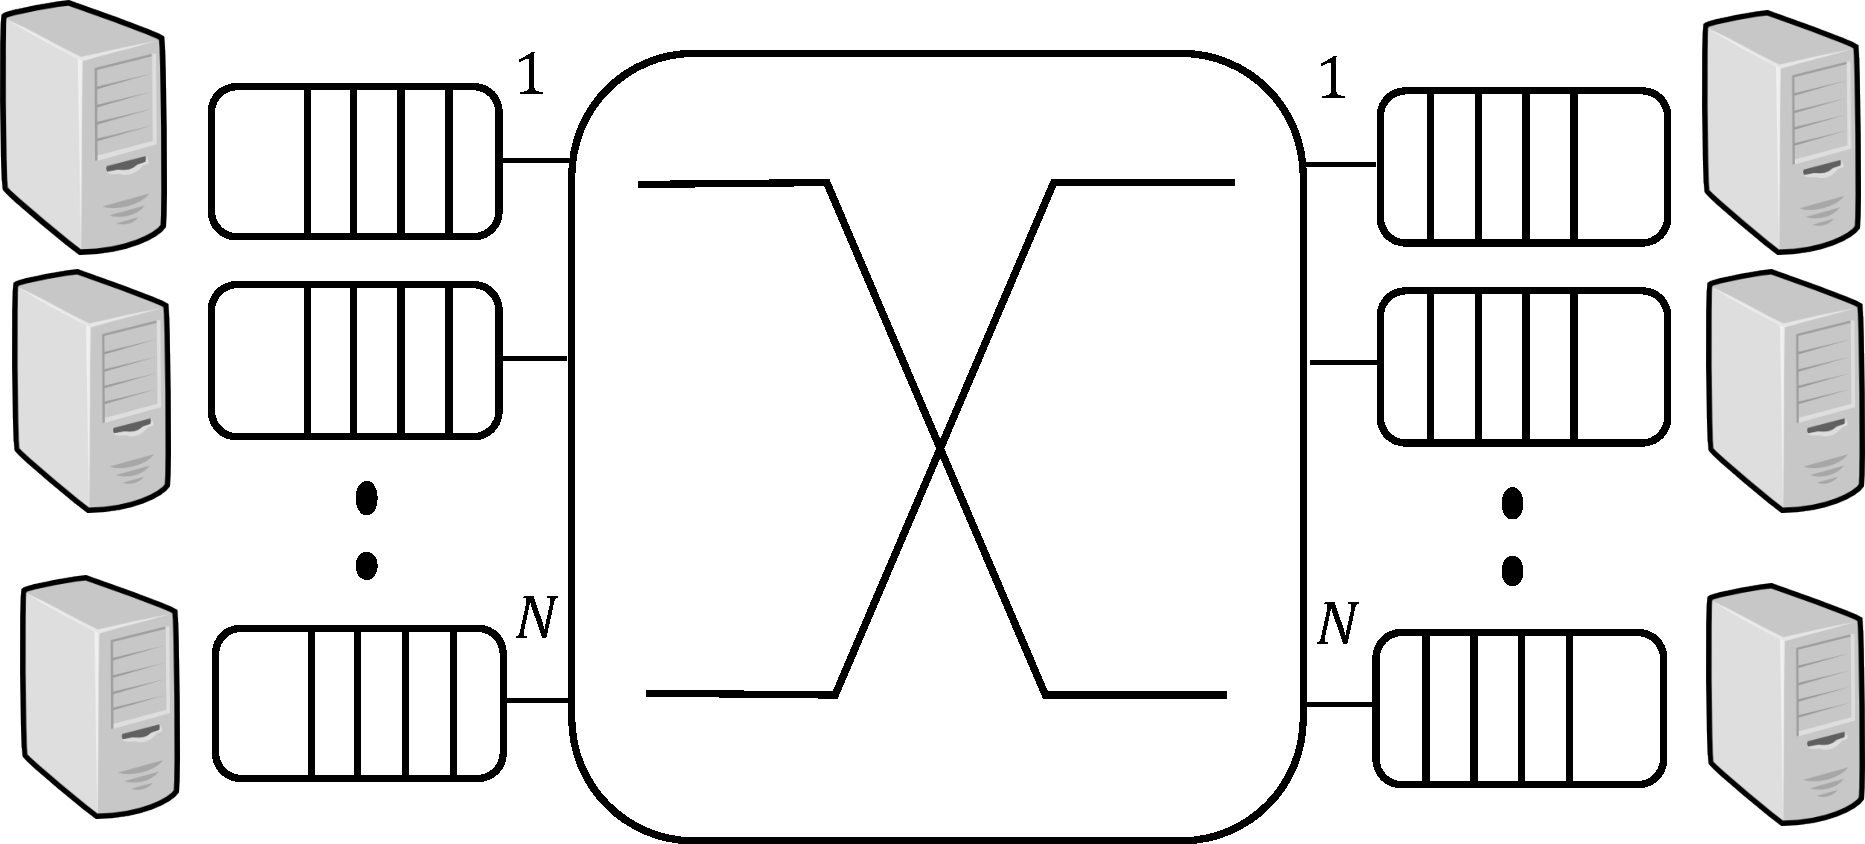
\includegraphics[width=0.55\textwidth]{Chapter2/Figures/pfabricdcn}
	\caption{Datacenter fabric abstraction as a giant switch}
	\label{fig:pfabricdcn}
\end{figure}

\subsubsection{Ideal flow scheduling in DCN}
Assuming that the fabric can sustain maximum throughput and that flows compete against each other only at ingress and egress interfaces, the optimal solution to minimize the flow completion time can be found solving a NP-hard problem known as \textit{sum-multicoloring}. Nevertheless, a simpler greedy algorithm exists and it has been proven to be very close to the optimum. Authors referred to this algorithm as the \textit{Ideal} algorithm and used it as a baseline for the evaluation of pFabric.  Briefly, it consists in a maximal flow scheduling, where at every new flow arrival or depart, flows are sorted in ascending order of data remaining up to their completion and served with this order. Flows are not served until there is another flow with less data remaining traversing the same ingress or egress port. Despite being a simplified model, still the \textit{Ideal} algorithm is a valid benchmark for any design that targets flow completion time minimization, since it is a sort of best case latency at a desired level of load and over an ideal interconnection network. \\
At this point, pFabric showcased that it is possible to achieve nearly ideal performances in a distributed way, treating each interface on its own with local scheduling decisions and simultaneously rely on minimal transport strategies. In particular, their work can be summarized in the following key aspects. \\
\begin{enumerate}
	\item \textit{Knowledge of flow requirements}. It is assumed to know at transport layer flow sizes or flow deadlines for deadline-constrained traffic. 
	\item \textit{Prioritization}. Schedulers in the network are priority schedulers. Depending on the scheduling objective, the packets encode with a priority a different metric, on which the scheduler choices are based on. For example, to approximate SRPT on every single link, the priority may indicate the amount of bytes still to transmit for a given flow. Packets are dequeued and dropped according to their priority. 
	\item \textit{Simple rate-control}. Rate control at end hosts is minimal and aims just to avoid persistent congestion. In fact, contrary to DCTCP (Sec. \ref{sec:dctcp}), even if queue sizes grow, only the performance of few long flows is significantly impacted, since it is used a detailed prioritization mechanism both for packet transmission and drops. Some shrinkage to standard TCP have been described to realize such minimalistic transport.
\end{enumerate}
 
 \subsubsection{Approximate optimality with priority queues}
As already mentioned, implementing such a prioritization scheme on available commodity devices is very challenging and for sure would require hardware modifications. The interested reader could find a possible digital design in the paper of pFabric. The same source, however, provided also a straightforward solution readily deployable with current switches. The idea is to coarse the granularity of the scheduler by adopting only a finite number of priority levels. Then, packets with different priorities are enqueued in corresponding priority queues (PQs) and handled with traditional network schedulers (SP, WRR, WFQ, etc.). In pFabric it is employed a Strict Priority (SP) scheduler, but in general other choices are not precluded \cite{mqecn}. In short, LAS and SRPT schedulers, as well as other disciplines, can be emulated by tagging packets with a priority label and leveraging separated queues in network interfaces. The typical number of priority queues available in datacenter switches ranges between 2 and 8, albeit it often occurs that some of them are reserved --- more details in Sec. \ref{sec:pias}. Of course, increasing the number of PQs results in better approximation of the ideal scheduling, that implicitly would correspond to having an infinite number of PQs. In fact, the ideal scheduler directly compares each other all priorities of the packets in the buffer.

Finally, the FCT gain obtained with this system largely depends on the way flows are clustered in priority levels. This underlies the need of a careful tuning of a set of thresholds which split packets among the priorities available. A dedicated section of this work illustrates some criterion to choose them (\S \ref{sec:thresholds}). 

\end{subsection}

\begin{subsection}{PIAS: the reference model}
	\label{sec:pias}
	The next step with respect to pFabric as well as the starting point of this work is PIAS: Practical Information-Agnostic Scheduler \cite{pias}. This proposal is the first which addresses the scheduling problem without the assumption of an exact prior knowledge about the flow size. Instead, PIAS tries to mimic a LAS scheduler exploiting the sole knowledge of the distribution of flow sizes rather than their precise values. Surprisingly, when compared to pFabric it delivers very similar performances for short flows, that are the more critical ones (the gap is within 4.9\%). At the same time, however, PIAS preserves ease of deployment with the current switch hardware and the standard distributed congestion-control algorithms.
	Summarizing, the two main design principles of PIAS are:
	
	\begin{enumerate}
		\item \textit{Flow-agnostic}. It requires only the knowledge of DC-wide flow size distribution, which can be easily estimated once and updated dynamically. Authors do not account for any heterogeneity of the distribution across different racks \cite{facebook_dcn}, in what the problem would become quite difficult ot treat with analytical methods. Also dynamic changes of the distribution along time have been ignored, but the architecture is flexible enough to adapt to this case.
		\item \textit{Low complexity}. It should be compatible with legacy TCP/IP protocol stack and readily deployable without touching the hardware of existing devices.
	\end{enumerate}

	\begin{figure}
		\centering
		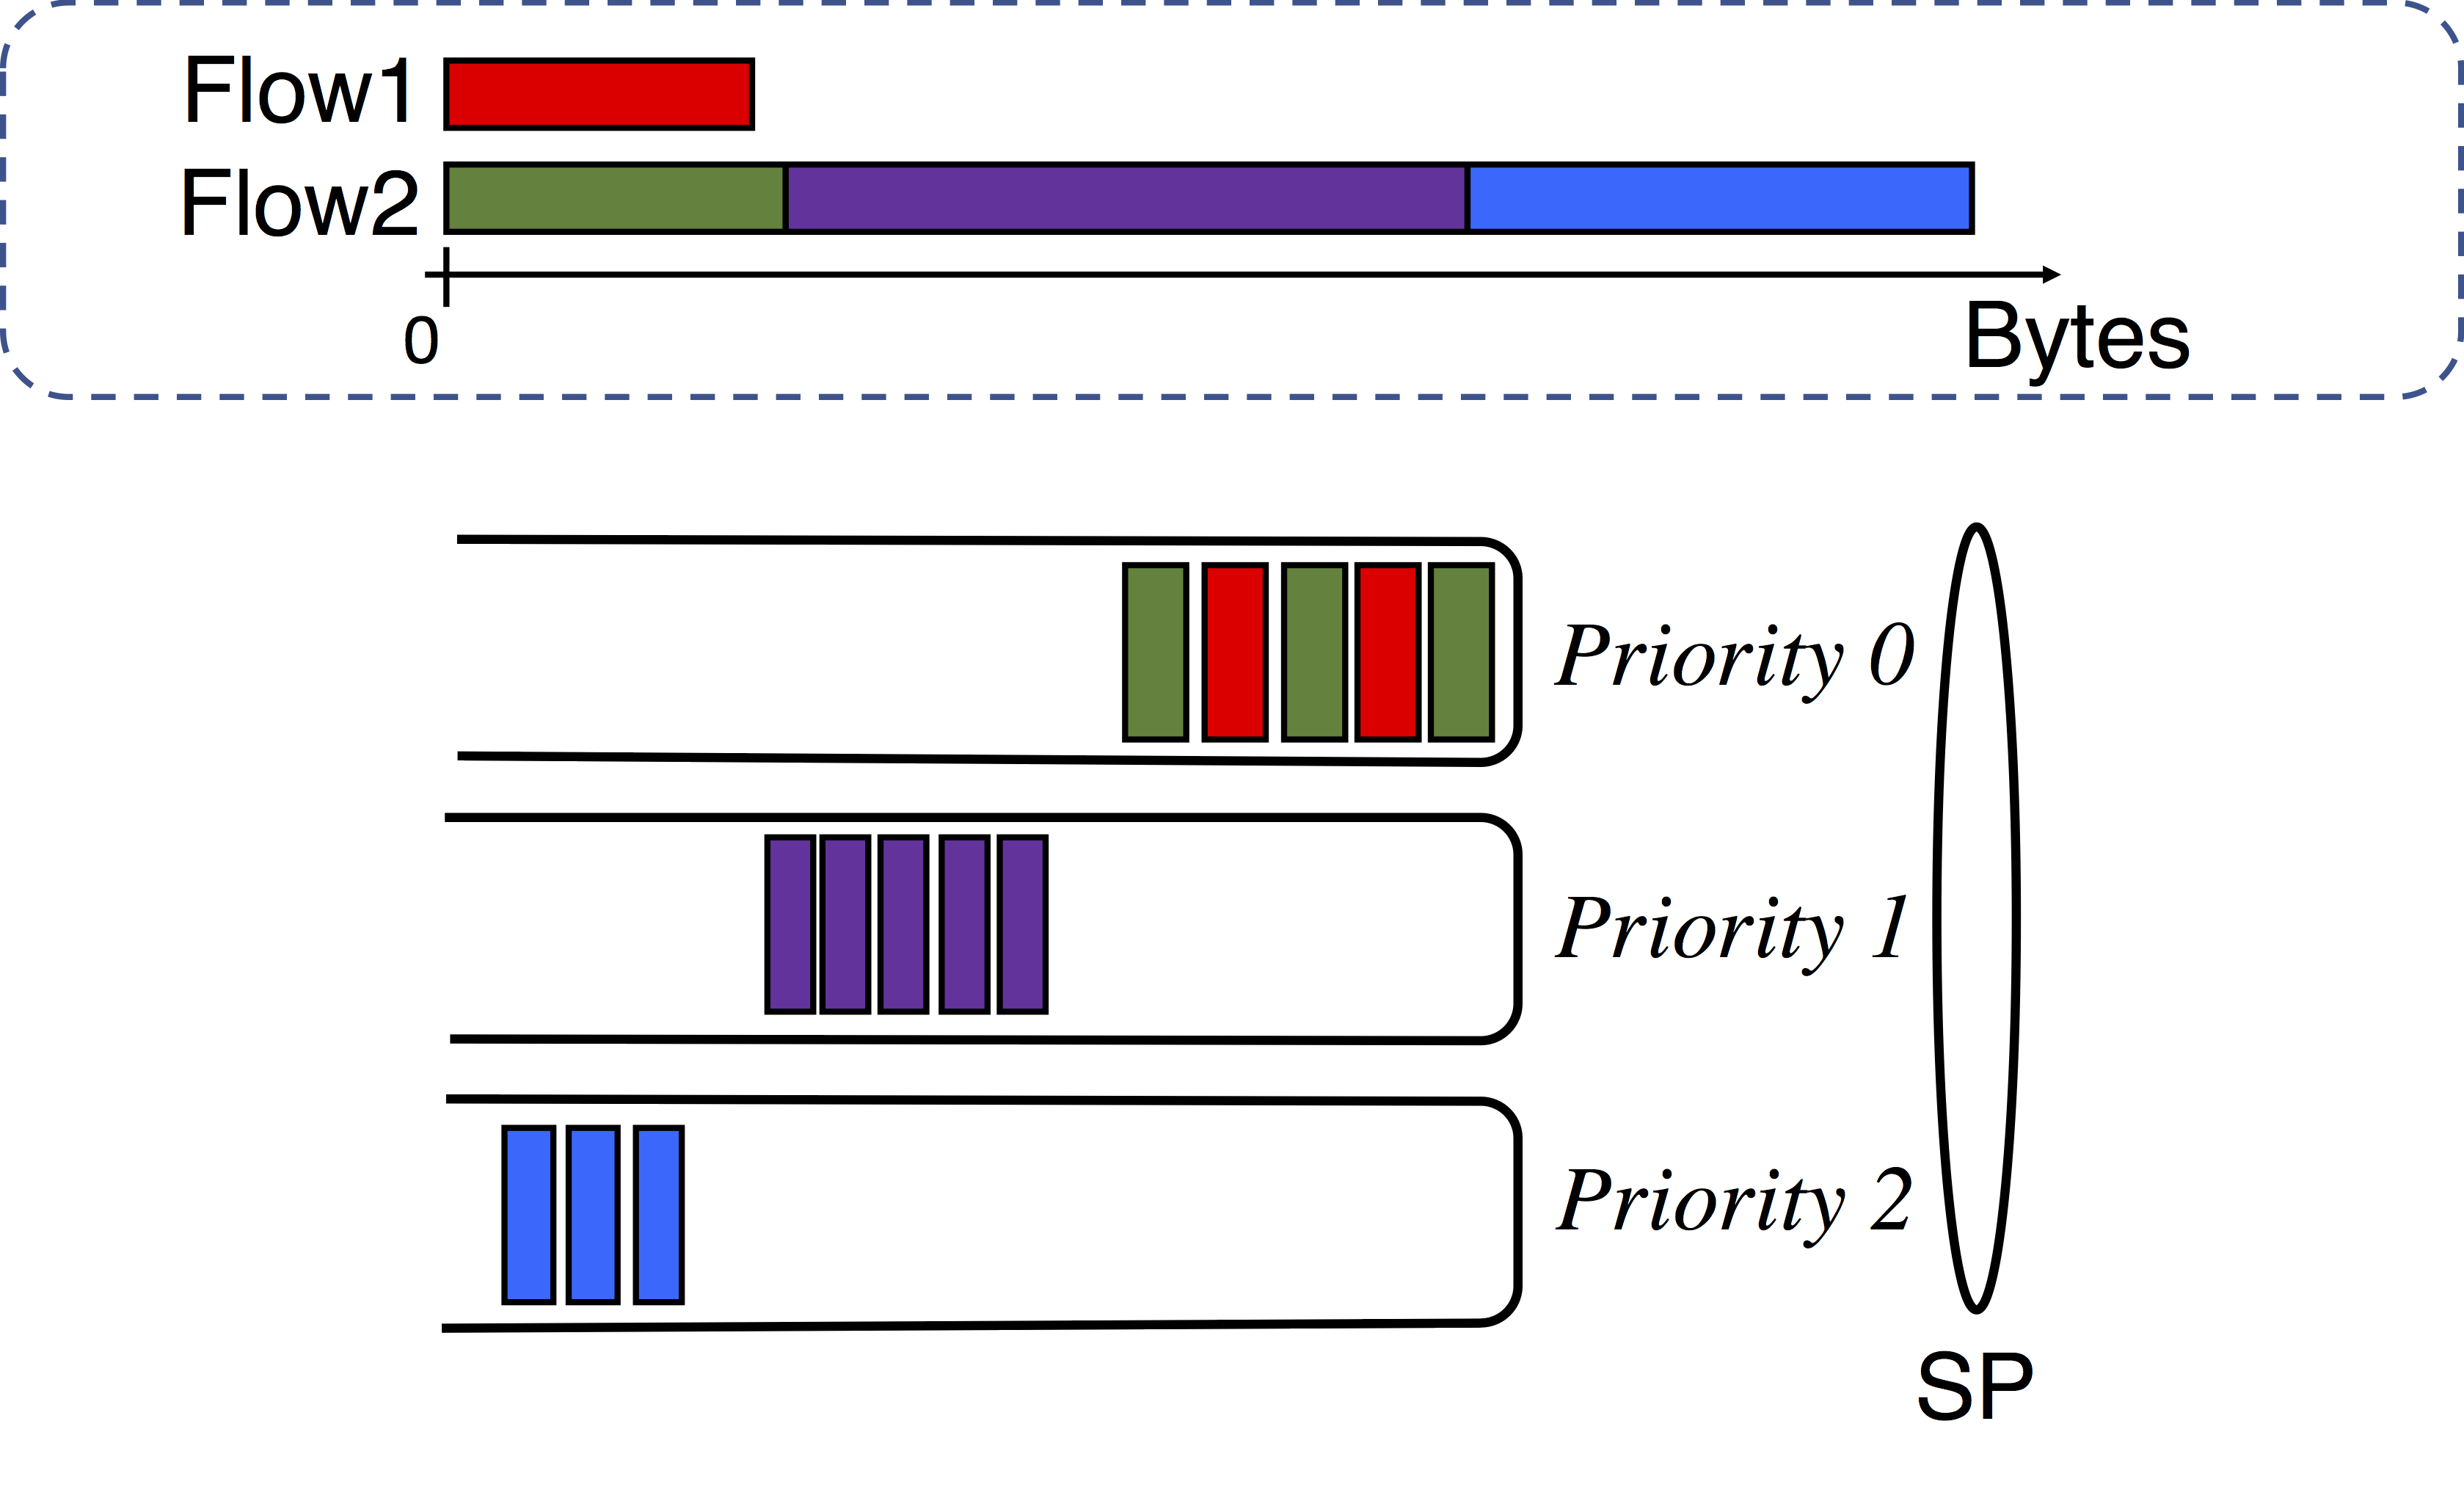
\includegraphics[width=0.5\textwidth]{Chapter2/Figures/pias_scheme}
		\caption{PIAS overview}
		\label{fig:pias_scheme}
	\end{figure}

	PIAS embraces a \emph{Multi Level Feedback Queue} (MLFQ) mechanism to resemble the LAS policy. MLFQ essentially apportion flows in a finite number of priority queues as proposed in pFabric, but in absence of flow size information flows are dynamically moved across priority queues. In more details, each packet of a given flow is mapped to a priority level, inversely proportional to the bytes it has already sent since its beginning. All flows starts with the highest priority, then longest flows are progressively demoted to lower priorities. Packets of same priority are buffered in the corresponding PQ according to a First-In First-Out (FIFO) order, while packets belonging to different priority queues are scheduled in Strict Priority (SP). In this way, packets belonging to short flows are always prioritized over those belonging to long flows, mimicking LAS but without incurring in the complexity of its implementation, which would require many comparisons. Figure \ref{fig:pias_scheme} clarifies the demotion mechanism. $\text{\emph{Flow}}_1$ is a mice flow and it is entirely served at the highest priority, whereas $\text{\emph{Flow}}_2$ is an elephant flow and it is gradually de-prioritized up to the last PQ. Notice that differently from pFabric, all flows traverse highest priorities in their initial lifetime, since their size is initially obscure. Hence, longer jobs constitute a small impairment for short ones, that motivates the gap with pFabric.

A key point for this kind of systems is how to choose the demotion thresholds. In fact, especially when few queues are available, an unbalanced threshold setting may lead to severe performance degradation. On one hand, thresholds too small cause premature flow demotion and delays for short flows that get mixed with long flows, on the other hand if the thresholds are too large, medium and elephant flows overstay in high priorities, resulting again in worse FCT for delay sensitive flows. The next section will present simple heuristics and a more refined optimization to find the set of thresholds.
\end{subsection}

\section{The problem of demotion thresholds}
The same authors of PIAS proposed a queueing model to mathematically describe the dynamics of the system. It has to be remarked that the queueing model captures only the average flow completion time on a single interface. Therefore, it is assumed that the flow size distribution is homogeneous over the datacenter fabric so that bottleneck links observe all the same distribution. With this assumption, the average FCT over the whole fabric is just a linear rescaling of the average FCT on a single link, therefore the performance index of any set of thresholds obtained with the model is meaningful for the whole DCN as well. 

In the following of this section, first it is formalized the queueing model along with its parameters, then it is formulated a non-linear minimization problem that can be used to optimize demotion thresholds. Finally, two other trivial heuristics for threshold assignment are reviewed.

\subsection{Stochastic queueing model}
\begin{figure}
	\centering
	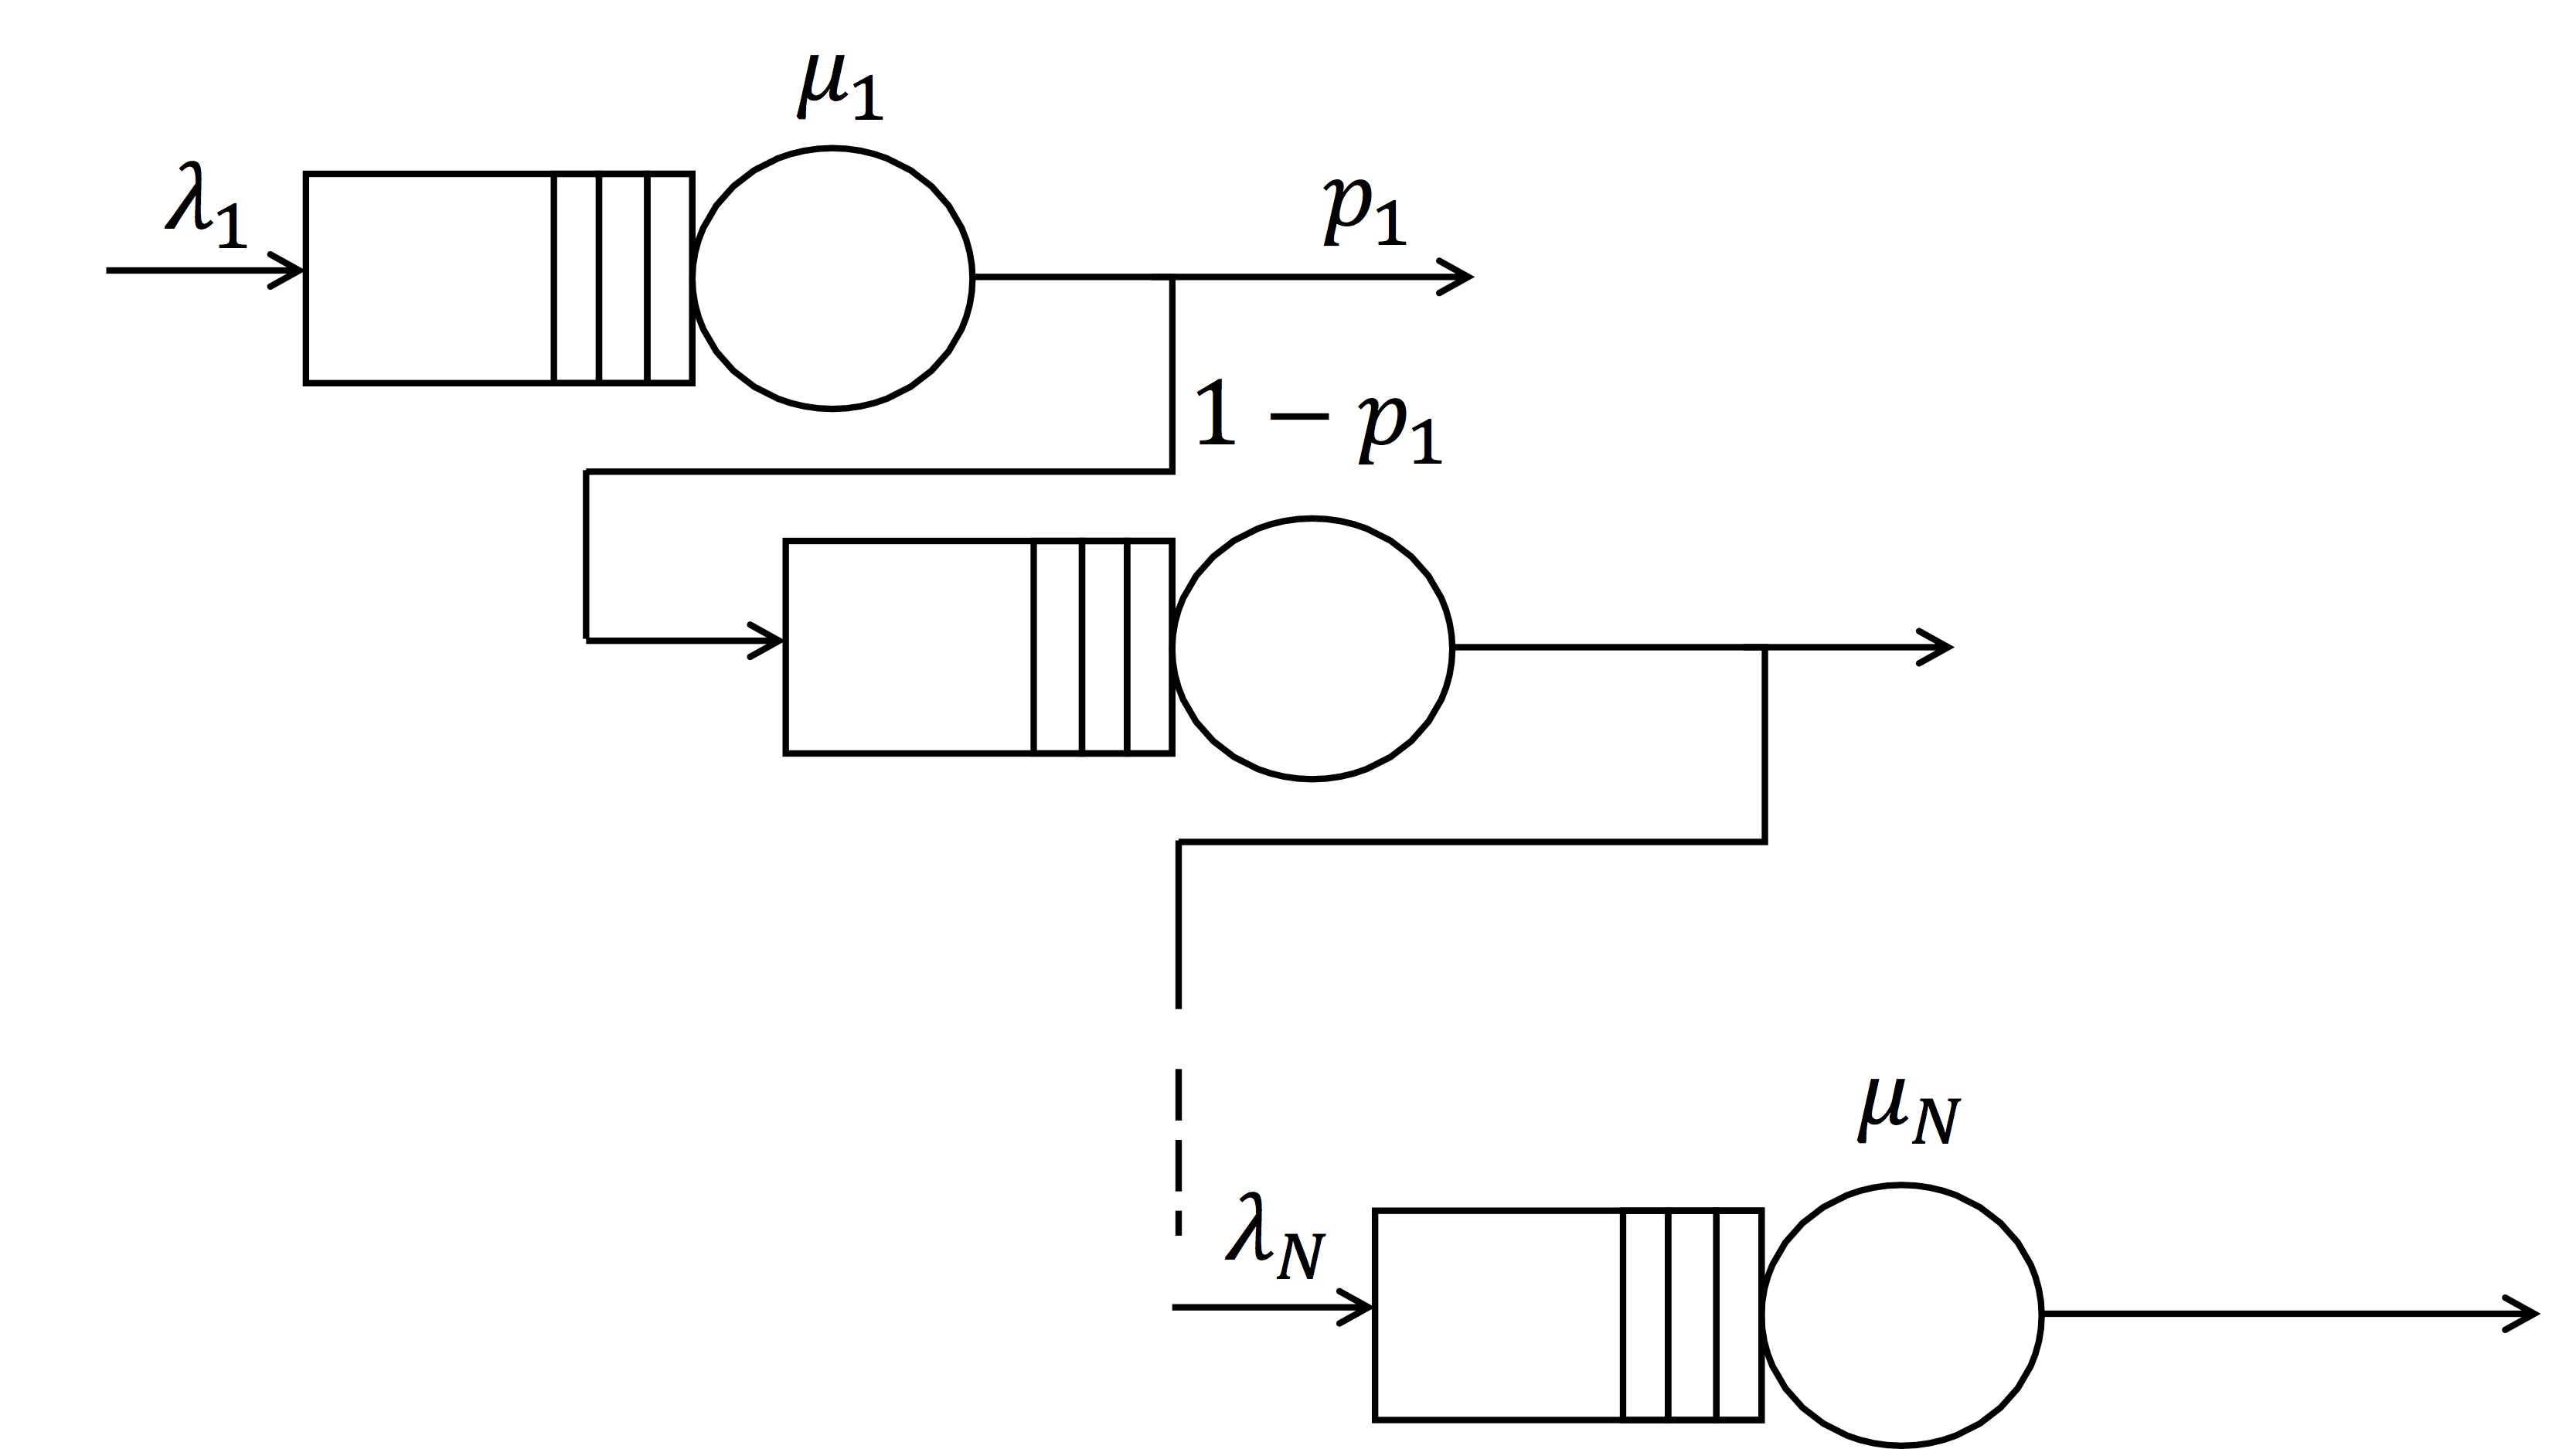
\includegraphics[width=0.5\textwidth]{Chapter2/Figures/pias}
	\caption{Queueing model}
	\label{fig:pias}
\end{figure}

The system, shown in Figure \ref{fig:pias}, is thought as a tandem of $N$ subsequent M/M/1 queues.  The customers are flows of size $X$ extracted from a given distribution with cumulative function $F(x)$ and arriving according to a Poisson process of intensity $\lambda$. Queues are lazy and able to serve at most a maximum amount of bytes for each flow, that depends on the demotion thresholds. When customers enter the system they are initially served by the first queue, then either they leave the system if all of their bytes have been served, or they are demoted to subsequent queue, up to queue $N$. \\ 
Let be $Q_p(1 \le p \le N)$ the $N$ priority queues. Denote with $\alpha_i$ the threshold after which a flow changes its priority from $i-1$ to $i$, where higher priorities correspond to lower indexes and $i \in [0,N]$. The upper threshold is always set to $\alpha_N = \infty$ so that all the largest flows stay in the last queue, similarly $\alpha_0 = 0$ for simplicity. Each queue $Q_i$ can serve at most $\alpha_i - \alpha_{i-1}$ bytes of any customer. In the real MLFQ system (Sec. \ref{sec:pias}), all queues of a given port are orchestrated by a Strict Priority (SP) scheduler, however this would make the queues dependent on each other complicating the analysis. To avoid the issue, the queues are treated as if they are independent and their priority hierarchy is taken into account by adjusting their drain rate $\mu_i$. In fact, if $\mu$ is the overall link capacity, subsequent queues in the tandem are assigned a drain rate $\mu_i$ equal to the residual bandwidth left after servicing previous queues. In practice, denote with $\rho_i$ the load insisting on $Q_i$, then 
\begin{equation}
\mu_i = \mu \prod_{j=1}^{i-1} (1-\rho_j)
\end{equation}
Next, for the sake of conciseness let's indicate with $\theta_i \triangleq F(\alpha_{i}) - F(\alpha_{i-1})$ the probability that a new flow has size in $[\alpha_{i-1}, \alpha_{i})$ and abbreviate with the notation $\bar{F}(x) = 1 - F(x)$ the survival function of $X$. The target is to derive the subsequent arrival rates $\lambda_i$.
After service in queue $i$, a customer leaves the system with a probability $p_i$, that depends on flow size distribution. In fact, customers who leaves the systems after the $i$-th queue are the flows with size in $[\alpha_{i-1}, \alpha_{i})$, among those with size in $[\alpha_{i-1}, \infty)$. Therefore, $p_i$ can be expressed renormalizing the probability $\theta_i$ as:
\[
p_i = \theta_i \mslash \bar{F}(\alpha_{i-1})
\]
Consequently, from the definition of $\theta_i$
\[ 	
1-p_i = \bar{F}(\alpha_{i}) \mslash \bar{F}(\alpha_{i-1}) 
\]
If the system is stable, the arrival rate of queue $i$ is nothing else than the output rate
of queue $i-1$, weighted by the probability of remaining in the system. 
Therefore: 
\[
\lambda_i = \lambda_{i-1} (1-p_{i-1})
\]
By iterative substitution it is possible to get a general expression for every $\lambda_i$ that depends only on the flow generation intensity $\lambda$ and the arrival rate at the previous queue $\lambda_{i-1}$. Indeed:
\begin{align*}
&\lambda_1 = \lambda \qquad \qquad & 1-p_1 &= \bar{F}(\alpha_1) / \bar{F}(\alpha_0) = \bar{F}(\alpha_1) \\
&\lambda_2 =  \lambda_1 (1-p_1) = \lambda \bar{F}(\alpha_1)  \qquad \qquad & 1-p_2 &= \bar{F}(\alpha_2) / \bar{F}(\alpha_1) \\
&\lambda_3 =  \lambda_2 (1-p_2) = \lambda \bar{F}(\alpha_2)  \qquad \qquad & 1-p_3 &= \bar{F}(\alpha_3) / \bar{F}(\alpha_2) \\
& \cdots \qquad \qquad & \cdots &
\end{align*}
In general:

\[
	\lambda_{i} = \lambda \bar{F}(\alpha_{i-1})
\]
Finally, this rate refers to flow arrivals, whereas thresholds $\alpha_i$ are expressed either in bytes or in packets, because they serve for demotion. It is simple to obtain the byte arrival rate by scaling $\lambda_i$ (flows/sec) of the average traffic size produced by these flows on queue $i$. Remember that due to the demotion mechanisms, customers of each queue are truncated versions of the original flows, whose size ranges in $(0, \alpha_{i}-\alpha_{i-1})$. and that, subsequent priority queues observe a flow distribution truncated above $\alpha_{i-1}$. \\
It is needed to compute $\mathbb{E}[L_i]$, the average length of customers served in queue $i$. It holds:

\begin{equation}
\label{load-on-pqi}
\mathbb{E}[L_i]=
\underbrace{\int_{\alpha_{i-1}}^{\alpha_i}(x-\alpha_{i-1})f(x)dx}_{\text{(i)}} +
\underbrace{(\alpha_{i}-\alpha_{i-1})\int_{\alpha_i}^{\infty}f(x)dx}_{\text{(ii)}}
\end{equation}

\begin{itemize}
	\item[(i)]Traffic generated by flows with sizes in $[\alpha_{i-1},\alpha_{i})$
	\item[(ii)] Traffic generated by flows larger than $\alpha_{i}$
\end{itemize}
Define the truncated probability density function seen by queue $i$ as:
\[
f_i(x) = f(x) \mslash \bar{F}(\alpha_{i-1})
\]
It holds:
\begin{equation}
\lambda_i =   \lambda \, \bar{F}(\alpha_{i-1}) \frac{\mathbb{E}[L_i]}{\bar{F}(\alpha_{i-1})} = \lambda \, \mathbb{E}[L_i]
\end{equation}

\begin{table}%[tb!]
	\label{tab:queuingmodel}
	\footnotesize 
	\centering
	\resizebox{0.6\textwidth}{!}{
		\begin{tabular}{c l l }
			\hline
			\textbf{Variable} & \multicolumn{1}{c}{\textbf{Description}}  \\ \hline \hline
			$Q_i$ & Priority queue $i$ \\ \hline
			$N$ & Number of priorities $i$ \\ \hline
			$X$ & Flow size \\ \hline
			$F(x)$ & Flow size c.d.f. \\ \hline
			$f(x)$ & Flow size p.d.f.  \\ \hline
			$\lambda_i$ & Packet arrival rate at PQ $i$  \\ \hline
			$\mu_i$ & Drain rate of PQ $i$ \\ \hline
			$\rho_i$ & Average load on $Q_i$ \\\hline
			$L_i$ & Customer size at PQ $i$   \\\hline
			$T_i$ & Waiting time at PQ $i$  \\\hline 
			$\alpha_i$ & Demotion threshold from $Q_{i-1}$ to $Q_i$ \\ \hline
			$p_i$ & Probability that a flow leaves after $Q_i$ \\ \hline 
			\hline
	\end{tabular}
}
	\caption{Variables of the model.}
\end{table}

Summarizing, it was possible to write down all arrival rates $\lambda_{i}$ and all draining rate $\mu_i$ as function of the flow size distribution and the set of thresholds $\alpha_i$. A summary of all quantities that have been defined is provided in Table \ref{tab:queuingmodel}.
These parameters are sufficient to express the average sojourn time on a single link, so to characterize the performance of PIAS. The average sojourn time on queue $i$ which comprises the average waiting and serving time is given by the well-known formula for M/M/1 queues:
\begin{equation}
\label{mm1}
\mathbb{E}[T_i] = \dfrac{1}{\mu_i-\lambda_i}
\end{equation}
The M/M/1 model holds for every subsequent queue. This follows from Burke's theorem \cite{burke}, that states that the outgoing process of an M/M/1 queue is a Poisson process. Thus, cascaded queues still observe a Markovian arrival process. \\
Finally, the total average sojourn time in the tandem of $N$ queues is just a linear combination of $\mathbb{E}[T_i]$, where the coefficient that weight the individual sojourn times at any priority queue are the probabilities that a flow shall traverse the same PQ.
\begin{equation}
\mathcal{T} = 
\sum_{i=1}^{N} \theta_i \sum_{j=i}^{N}\mathbb{E}[T_j]
\end{equation}
Thus, given the flow size distribution it is possible to easily compute the system performance according to the model yet presented. 

\subsubsection{Optimal thresholds}
\label{sec:pias-queueing-model}
Plainly, it follows that the \textit{optimal} thresholds $\alpha_i$ can be derived solving the non-linear minimization of $\mathcal{T}$. Notice that they are easily obtainable once all $\theta_i$ are known as 

\[
\alpha_i = F^{-1}(\sum_{j=1}^{i}\theta_j)
\]
Hence, it is possible to solve in $\theta_i$.
\begin{equation}
\label{eq::costfunction}
\begin{aligned}
&\underset{\{\theta_i\}}{\text{min}} \quad  & &\mathcal{T} = 
\sum_{i=1}^{N} \theta_i \sum_{j=i}^{N}T_j \\
&\text{subject to} \quad  & &\theta_i \ge 0 \qquad \qquad \qquad \forall i \in [1,N]  \\
& & & \sum_{i=1}^{N} \theta_i = 1 
\end{aligned}
\end{equation}

\subsection{Greedy threshold assignment}
\label{sec:greedy-thresh}
In order to verify the actual gain obtained with optimal demotion levels, it is practical to compare it against simpler greedy strategies for thresholds assignment. Another reason motivating such alternatives is that when the number of priority levels increases ($N$>3) the solution to the previous optimization is very time consuming, since the problem is non-linear and non-convex. In chapter \ref{ch4} it is provided a breakdown which shows the CPU time spent for computing the optimal demotion thresholds through a meta-heuristic algorithm. 
Having a significant slow-down for the solution to converge deteriorates the reactiveness of the MLFQ scheduler in the case of a sudden change in the flow size distribution. As a consequence, the system would operate for long using thresholds mismatched with respect to the flow distribution.

Two intuitive approach are considered for fast threshold computation: Equal Split (ES) and Load Split (LS). 
%Therefore, for initial tests, it has been more practical to use a simpler criterion: assign thresholds so that the traffic load is equally distributed among available queues. \\

\subsubsection{Equal Split (ES-N)}
The \textit{Equal-Split} method slices the flow size distribution uniformly in $N$ percentiles. The resulting thresholds are the corresponding quantiles:

\[
\alpha_{i} = F^{-1}\Big(\dfrac{i}{N}\Big), \qquad i=1,..,N-1
\]
It is easy to observe that this criterion may be largely sub-optimal depending on the shape of the flow size distribution. In the case of very sharped distributions short flows are demoted too early to lower priorities, while for heavy-tailed distributions, where high percentiles correspond to very long flows, latency sensitive flows remains mixed for long with elephant throughput-oriented streams.

\subsubsection{Load Split}
\emph{Load Split} is a technique where the thresholds are chosen in a way to control the amount of traffic fed in every priority queue.  The problem is easy to understand in the simple case of $N$=2 priority queues and a single threshold $\alpha$. Let $G(y)$ be the amount of traffic generated by flows with size less than $y$:
\[
G(y) = \int_{0}^y x f(x) dx
\]
The traffic on high priority queue $Q_0$ is derived as the sum of bytes generated by flows whose size is smaller than the threshold $\alpha$, and the bytes transmitted by flows larger than $\alpha$:
\[
\mathbb{E}[L_0] = \int_0^\alpha xf(x)dx+\int_\alpha^\infty \alpha f(x) dx=G(\alpha)+\alpha \bar{F}(\alpha)
\]
while the traffic on low priority queue is
\begin{equation*}
\mathbb{E}[L_1] =\int_\alpha^\infty (x-\alpha)f(x)dx=\mathbb{E}[X]-	\mathbb{E}[L_0]
\end{equation*}
Then, the traffic on the high priority queue can be controlled solving the following \textit{load-balance} equation:

\begin{equation}
\label{eq:main-gen}
\mathbb{E}[L_0] = \gamma \mathbb E[X] 
\end{equation}

A proper choice of $\gamma$ apportions to the high priority queue a fraction of the average total traffic $\mathbb{E}[X]  = \mathbb{E}[L_0] + \mathbb{E}[L_1]$. For example, if a perfect load balancing between the two queues is desired then it is set $\gamma = 1/2$.
Extending these equations to the general case of any number of priority queues is rather simple. The traffic on the $i$-th queue has the same expression of Eq\eqref{load-on-pqi}. It can be rewritten shortly with the notation just introduced:
\[
\mathbb{E}[L_i] = G(\alpha_i) - G(\alpha_{i-1}) + \alpha_i \bar{F}(\alpha_i) -\alpha_{i-1}\bar{F}(\alpha_{i-1})
\]
At this point, similarly to the simple case of two queues, it is enough to solve the following \emph{load-balance} equations iteratively for all $i = 1,..,N-1$:

\begin{equation}\label{eq:main-K-PQ}
\begin{cases}
\mathbb{E}[L_i] = \gamma_i \, \mathbb{E}[X],  \qquad &i = 1,..,N-1 \\
\sum_i \gamma_i = 1, \qquad &\gamma_i \in [0,1]
\end{cases}
\end{equation}
In fact, also in this case it holds $\sum_{i=1}^{N}\mathbb{E}[L_i] = \mathbb{E}[X]$.

\renewcommand{\qedsymbol}{\rule{0.5em}{0.5em}}
\begin{proof}
\label{proof}
\textit{In the expansion of $\sum _{i=1}^{N}\mathbb{E}[L_i]$ at each step new terms simplify old terms. Since $\alpha_{\mathit{0}} = 0$ and $\bar{F}(\alpha_N) = 0$, it gives $\int_{0}^\infty x f(x) dx = \mathbb{E}[X]$}.
\small
\begin{align*}
	\sum\nolimits_{i=1}^{N}\mathbb{E}[L_i] &= \cdots + \cancel{G(\alpha_i)} - G(\alpha_{i-1}) + \cancel{\alpha_i \bar{F}(\alpha_i)} 
	-\alpha_{i-1}\bar{F}(\alpha_{i-1}) + G(\alpha_{i+1}) - \cancel{G(\alpha_{i})} \\ &+ \alpha_{i+1} \bar{F}(\alpha_{i+1})- \cancel{\alpha_{i}\bar{F}(\alpha_{i})} + \cdots 
	=G(\alpha_N) - G(\alpha_0) + \cancelto{0}{\alpha_N \bar{F}(\alpha_N)} -\cancelto{0}{\alpha_0\bar{F}(\alpha_0)} \\
	&=\mathbb{E}[X].
\end{align*}
\normalsize
\end{proof}

\section{A priority scheme with spatial-diversity}

\subsection{MLFQ with Spatial-Diversity}
In this chapter have been presented two attempts to approximate the optimal LAS and SRPT schedulers leveraging multiple priority queues, that are already present in all datacenter equipments. However, one limitation of this approach remains the scarce availability of priority queues in commodity switches. A large number of priority levels is demanded to better approximate the reference scheduling disciplines, in which $N \rightarrow \infty$ (Sec. \ref{sec:las}). Unfortunately, devices in modern DCNs are usually equipped with no more than 8 priority queues per port, whose majority are reserved for other purposes, like isolating different types of traffic. Indeed, several transport protocols may coexist in the same network, without necessarily being designed to be fair among them. Example of such transports are RDMA \cite{rdma}, DCTCP \cite{dctcp}, standard TCP and UDP. For this reason, it is plausible to assume to have at most $N=2$ priority queues as a realistic case. \\
Upon this understanding, the main proposal of this work is to evaluate the possibility to exploit the high degree of spatial diversity typically offered by DCN topologies to improve flow scheduling. Large DCN topologies are multilayer recursive Clos networks which offer a variety of equal-cost paths between racks. Precisely, in the simplest 2-layer Fat-Tree there are a number of paths proportional to the number of spines $K$ (Sec. \ref{sec:topology}). The key observation is that much like priority queues, different paths yet are a way for separating flows. In other words, the mechanism of priority demotion which shift the long flows across priority queues of a single interface, could be potentially applied at higher level as routing strategy over the switching fabric. Elephant flows would be physically segregated from mice flows, as they would be moved to different paths inside the switching fabric. Despite its simplicity, relevant works exploring this solution in the field of datacenter networks seem to be lacking. In more details, this contribution aims to integrate the spatial diversity property with the MLFQ scheduler. Consider a Leaf-Spine topology and focus on a single ToR switch. The interfaces from such a ToR towards all spines can be seen jointly as a unique big interface with $K$ times more priority queues than a port alone. The idea is better clarified in Fig.\ref{fig:sd-key-idea}.
\begin{figure}
	\centering
	\begin{subfigure}[htpb]{0.3\textwidth}
		\centering
		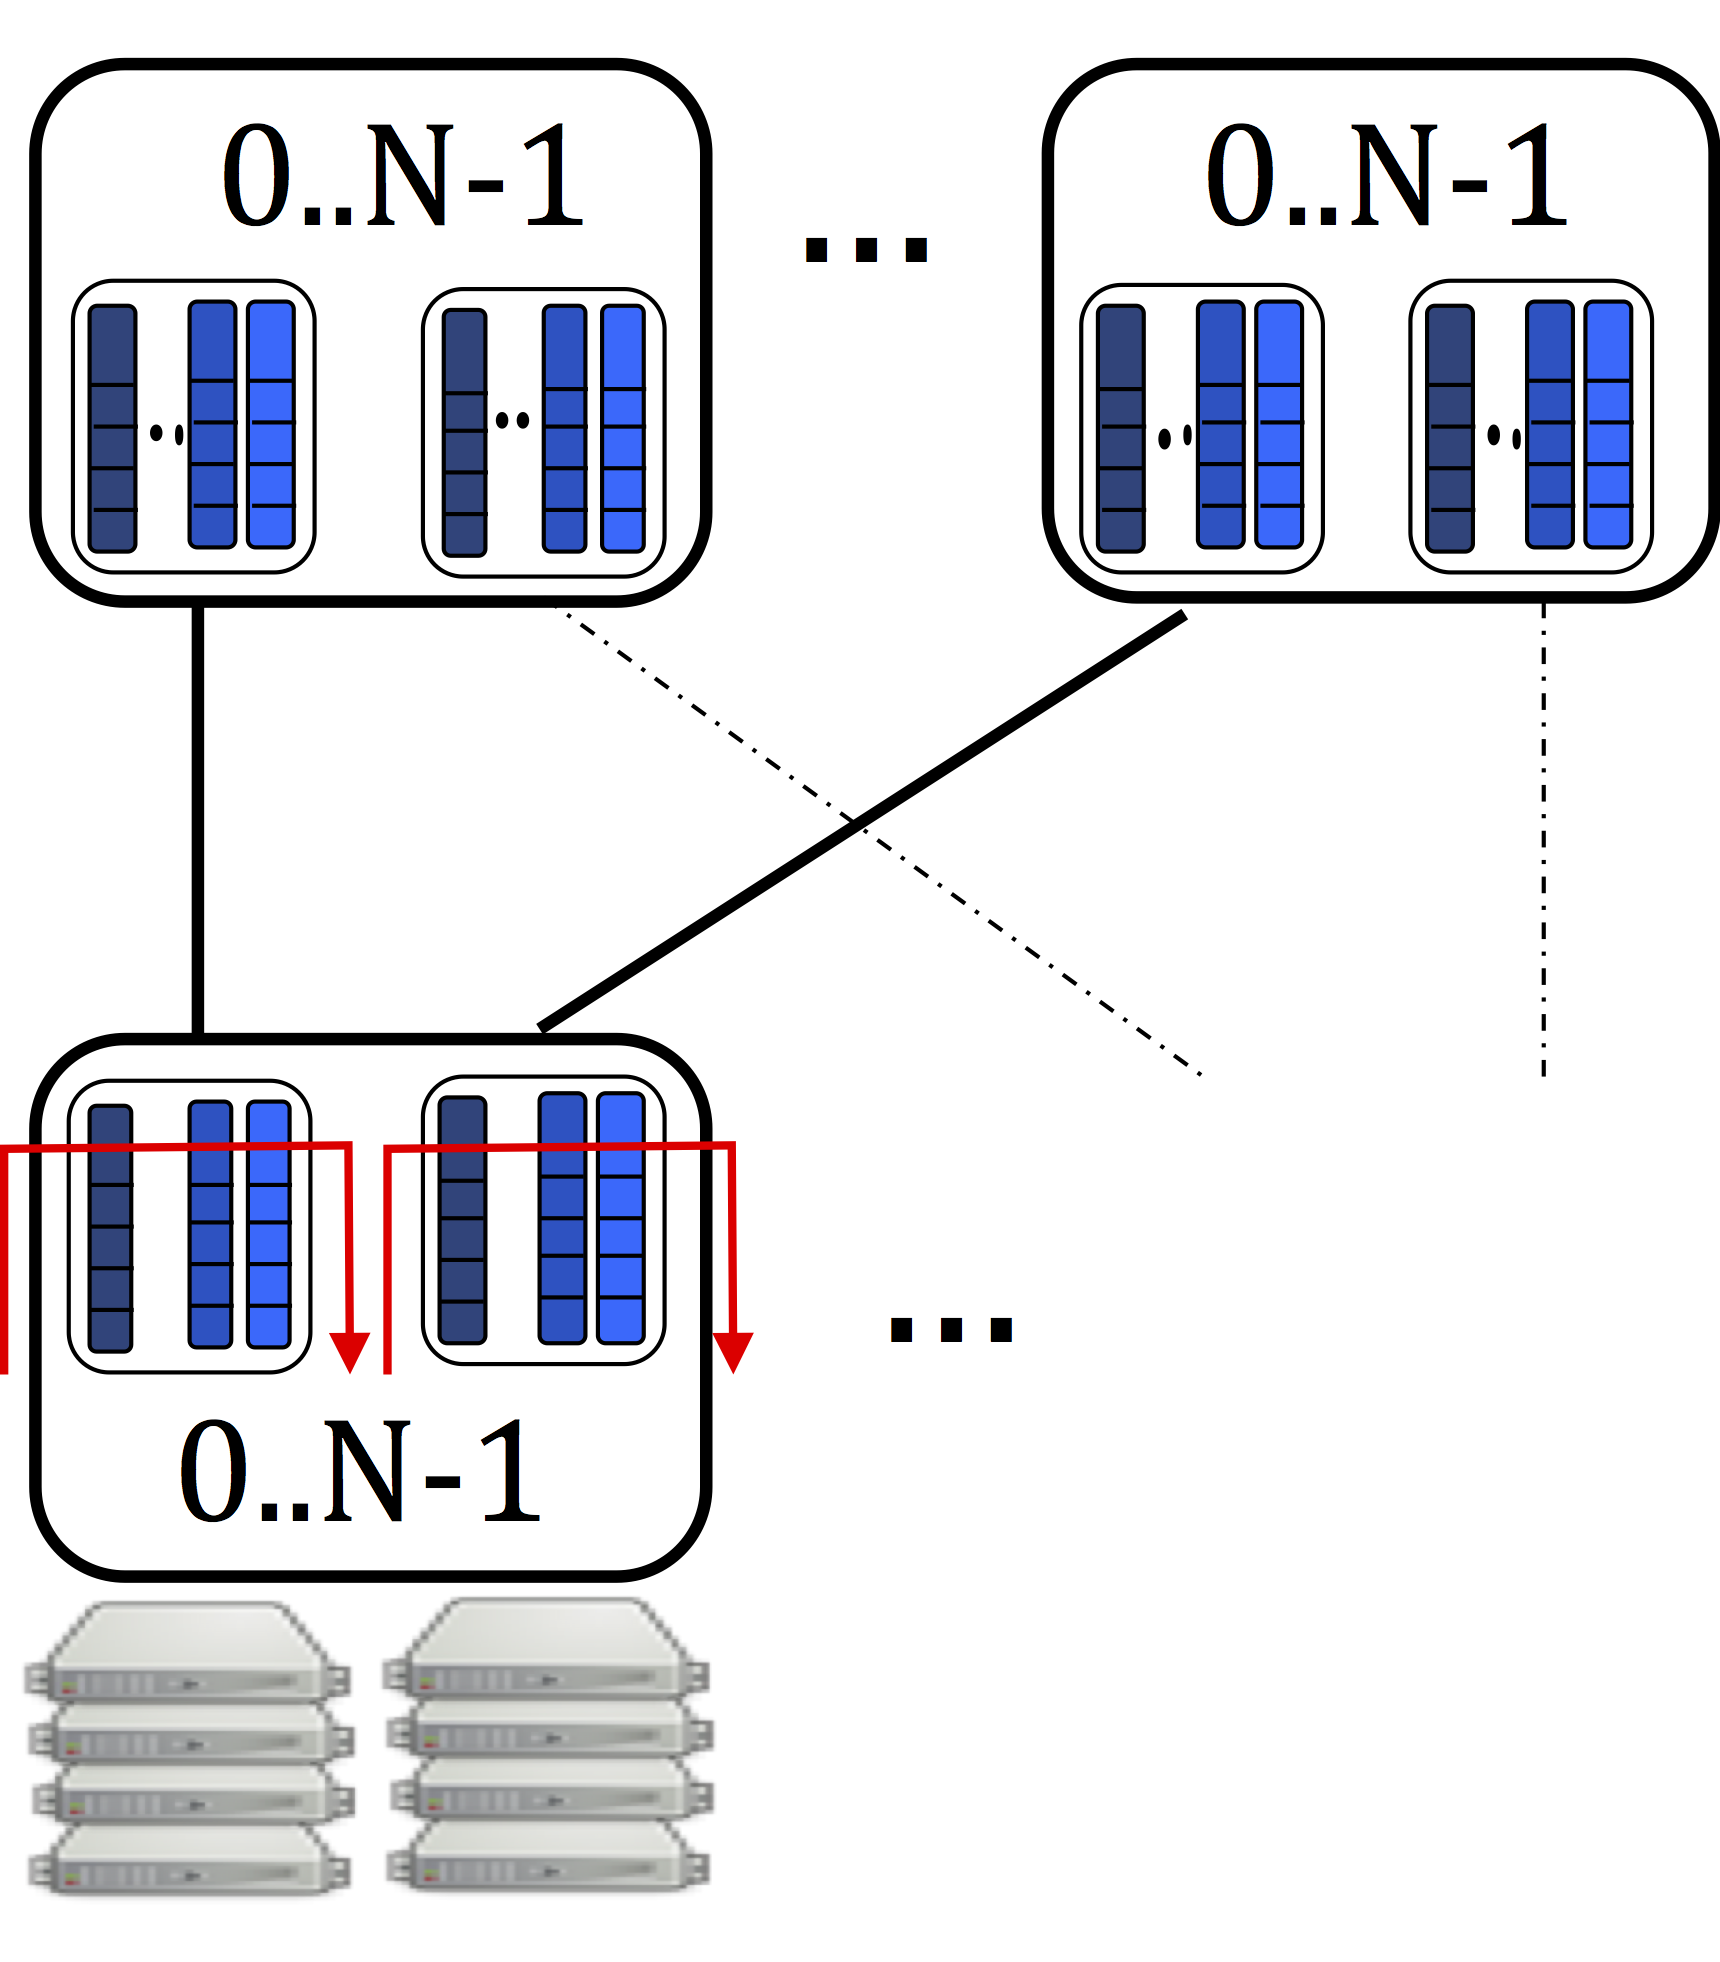
\includegraphics[width=\textwidth]{Chapter2/Figures/mlfq}
		\caption{MLFQ}
		\label{fig:sd-key-idea-mlfq}
	\end{subfigure}
	\hspace{0.2\textwidth}%
	\begin{subfigure}[htpb]{0.3\textwidth}
		\centering
		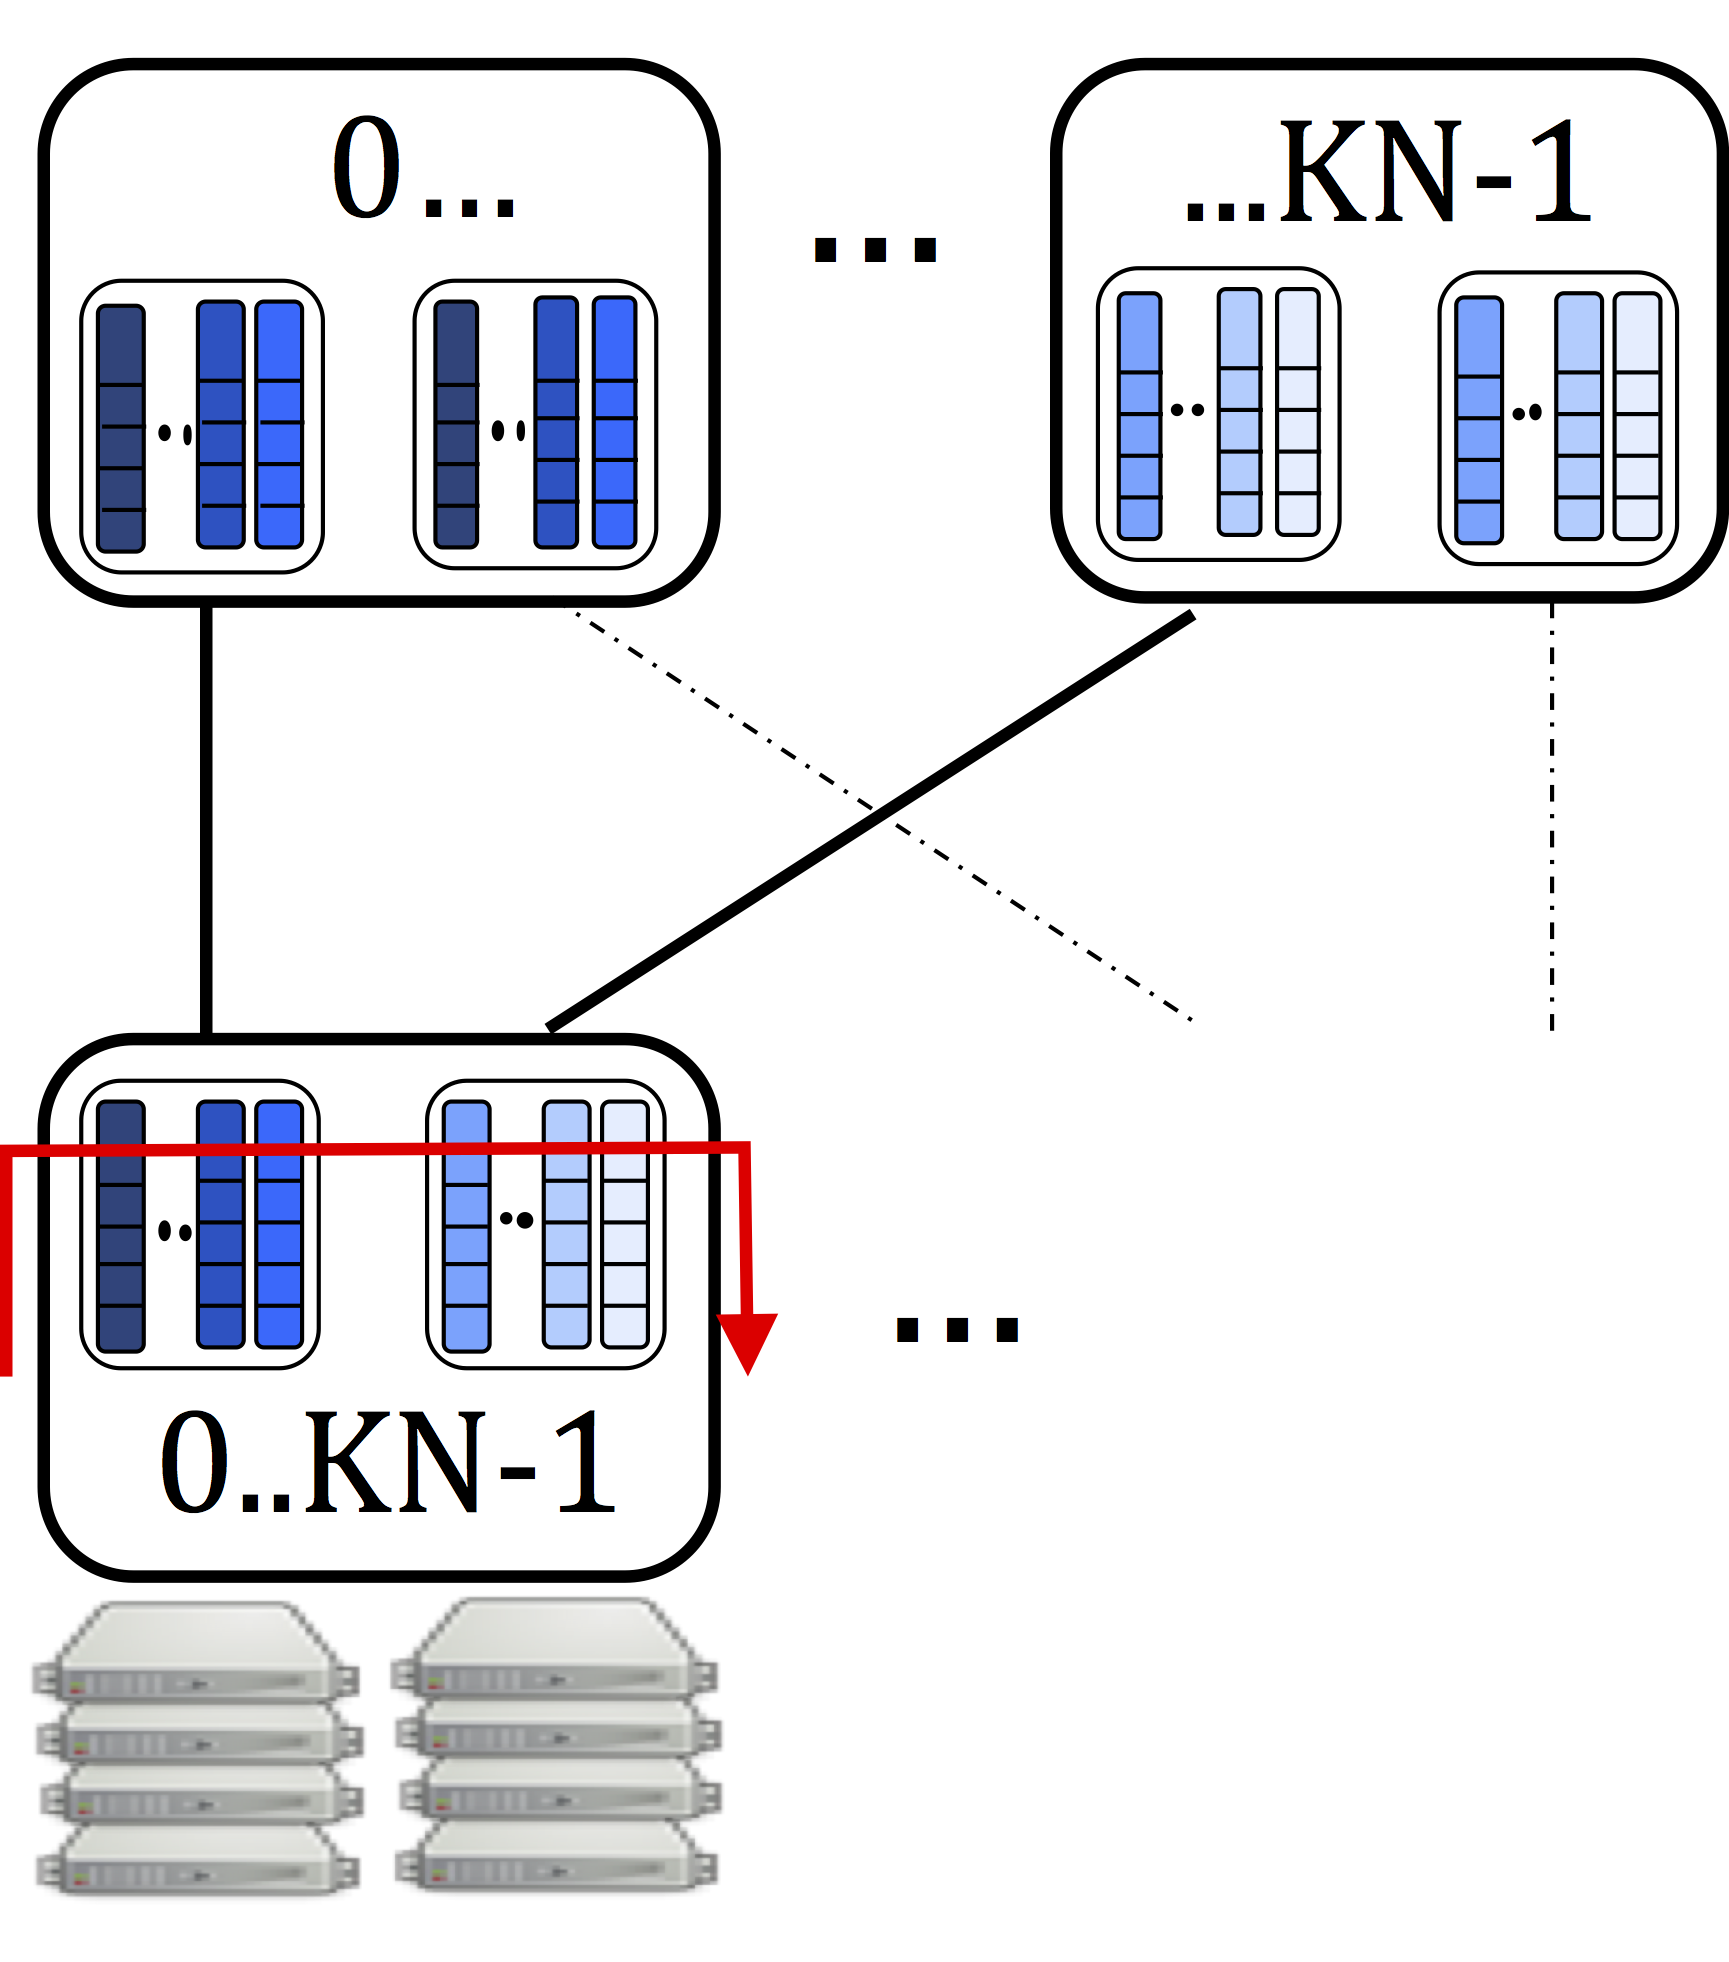
\includegraphics[width=\textwidth]{Chapter2/Figures/sdmlfq}
		\caption{SD-MLFQ}
		\label{fig:sd-key-idea-sdmlfq}
	\end{subfigure}
	\caption{Extension for spatial diversity.} %Red arrows indicate how queues are traversed during flow demotion. On each switch is reported the number of priorities it handles. Color scale is used to emphasize priority levels.}
	\label{fig:sd-key-idea}
\end{figure}
%Differently from 
The basic MLFQ (Fig.\ref{fig:sd-key-idea-mlfq}) focuses on the links individually and thanks to demotion moves flows, during their lifetime, across priority queues. Therefore, every interface handle the same priorities and flows are load balanced on different links independently from the prioritization mechanism. A standard technique for load balancing at flow-level is ECMP, which derives the next hop from the transport-layer tuple \texttt{\{IP ADDRESSES, PORTS, PROTOCOL ID\}}. Instead, this novel approach takes advantage of spatial diversity to extend the number of demotion levels beyond the limitation imposed by the PQs on a single interface. Interfaces from any ToR to the connected spines are virtually aggregated to offer a wider range of demotion levels. One new aspect of Spatially-Diverse MLFQ (SD-MLFQ) is that a demotion could imply to shift a flow from one path to another of equal-cost. In that light, the routing --- thus load balancing --- of flows on the Fat-Tree does depend on the priority. The spines can be seen as if they have a priority and a flow is moved both across queues and spines, effectively allowing a global resource exploitation for the demotion scheme. In other words, the routing policy over the fabric is not blind to the prioritization machinery, but smartly driven by the latter.  \\
A clear benefit of this scheme is that finer granularity in priorities is achieved even with few queues per port, at the price of a very limited implementation complexity.

\subsection{A queueing model extension for spatial-diversity}
\label{sec:complete-model}
PIAS model with added dimension for spatial diversity.
Proportional and equal splits for spatial diversiy
